%% bar_charts.tex
%% Author: Leighton Pritchard
%% Copyright: James Hutton Institute
%% Do bar charts misrepresent data?

% DISDAIN FOR BAR CHARTS
\begin{frame}
  \frametitle{Bar charts are bad$\ldots$mmmkay?}
  \textcolor{hutton_green}{There is an ongoing backlash against bar charts} \\
  (and I'm not picking on Nick, he just tweets a lot$\ldots$)
  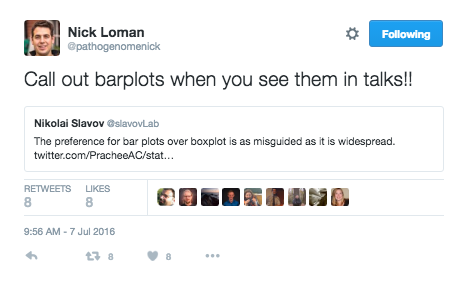
\includegraphics[height=0.3\textheight]{images/tweet_barchart}
  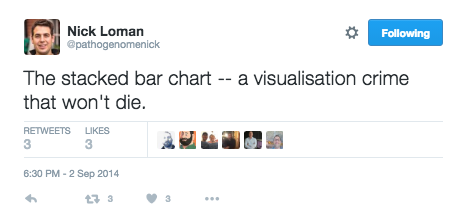
\includegraphics[height=0.3\textheight]{images/tweet_stackedbar} \\
  \textcolor{hutton_blue}{But are they really that bad?}
\end{frame}

% BAR/LINE INTERPRETATION 1
\begin{frame}
  \frametitle{Interpretation of bars and lines
  \footnote{\tiny{\href{http://link.springer.com/article/10.3758/BF03201236}{Zacks \& Tversky (1999) \textit{Mem. Cognit.}}}}
  }
  \begin{alertblock}{People interpret bars and lines differently}
  Experiment 1: In absence of context (arbitrary $X$, $Y$)
    \begin{itemize}
      \item \textbf{bars}: discrete comparison (24:0)
      \item \textbf{lines}: trend assessment (0:35)
    \end{itemize}
  \end{alertblock}
  \begin{center}
    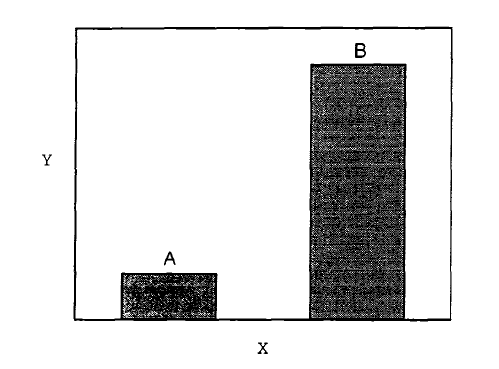
\includegraphics[width=0.4\textwidth,valign=t]{images/bars_v_lines_expt1a}    
    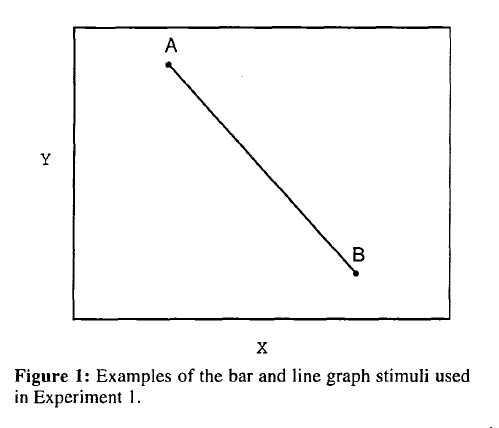
\includegraphics[width=0.4\textwidth,valign=t]{images/bars_v_lines_expt1b}  
  \end{center}
\end{frame}

% BAR/LINE INTERPRETATION 2
\begin{frame}
  \frametitle{Interpretation of bars and lines
  \footnote{\tiny{\href{http://link.springer.com/article/10.3758/BF03201236}{Zacks \& Tversky (1999) \textit{Mem. Cognit.}}}}
  }
  \begin{alertblock}{People interpret bars and lines differently}
  Experiment 2: With context (discrete or continuous data)\\
    \begin{center}
      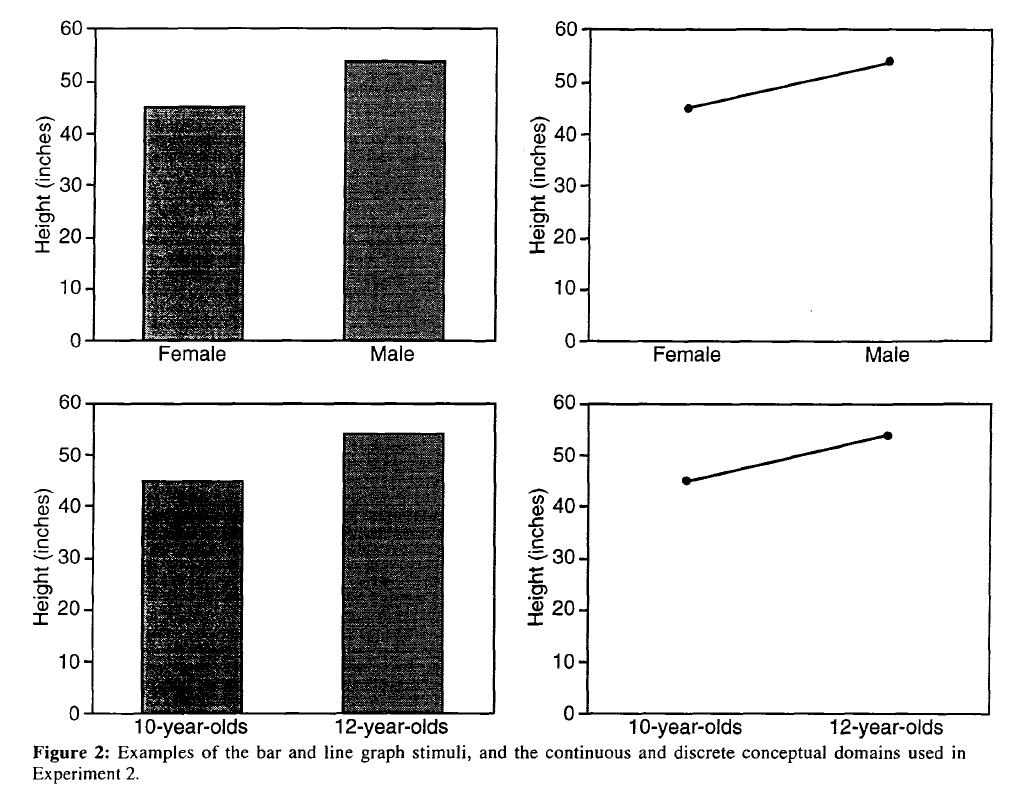
\includegraphics[height=0.4\textheight,valign=t]{images/bars_v_lines_expt2} \\
      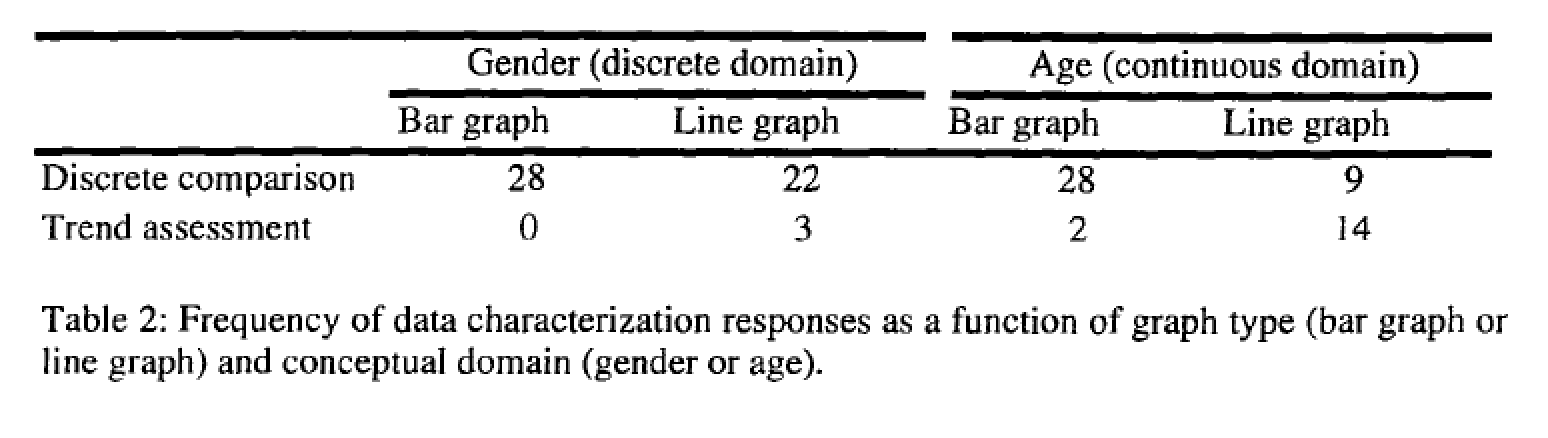
\includegraphics[width=0.7\textwidth,valign=t]{images/bars_v_lines_table}  
    \end{center}
  \end{alertblock}
  \begin{center}
  \end{center}
\end{frame}

% BAR/LINE CONCLUSIONS
\begin{frame}
  \frametitle{Bars \textit{ vs.} lines}
    \begin{itemize}  
      \item \textcolor{hutton_green}{People naturally interpret bar charts as categorical data}
      \item \textcolor{hutton_blue}{People naturally interpret line graphs as trends}
      \item \textcolor{hutton_purple}{Using bars for trend data or lines for categorical data can mislead the reader}
    \end{itemize}  
\end{frame}

% BAR CHARTS CAN MISLEAD
\begin{frame}
  \frametitle{Bar charts can mislead
  \footnote{\tiny{\href{http://dx.doi.org/10.1371/journal.pbio.1002128}{Weissgerber \textit{et al.} (2015) \textit{PLoS Biol.} doi:10.1371/journal.pbio.1002128}}}
  }
  \begin{columns}[T]
    \begin{column}{6cm}  
      \begin{itemize}  
        \item <1->\textcolor{hutton_green}{Do these bars differ in value?}
        \item <2->\textcolor{hutton_blue}{Bar charts represent data as a single point: lossy compression.}
        \item <2->\textcolor{hutton_purple}{Could different datasets give the same bar chart?}
      \end{itemize}  
    \end{column}
    \begin{column}{4cm}  
      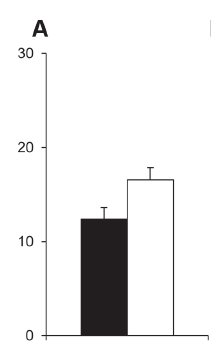
\includegraphics[width=1\textwidth]{images/weissgerber1}    
    \end{column}
  \end{columns}   
\end{frame}

% BARS ARE LOSSY COMPRESSION
\begin{frame}
  \frametitle{Bars are lossy compression
  \footnote{\tiny{\href{http://dx.doi.org/10.1371/journal.pbio.1002128}{Weissgerber \textit{et al.} (2015) \textit{PLoS Biol.} doi:10.1371/journal.pbio.1002128}}}
  }
    \begin{alertblock}{Bars hide detail:}
      \begin{itemize}
        \item Number of data points
        \item Variance of data points
        \item Distribution of data points (outliers, etc.)
      \end{itemize}
    \end{alertblock}
    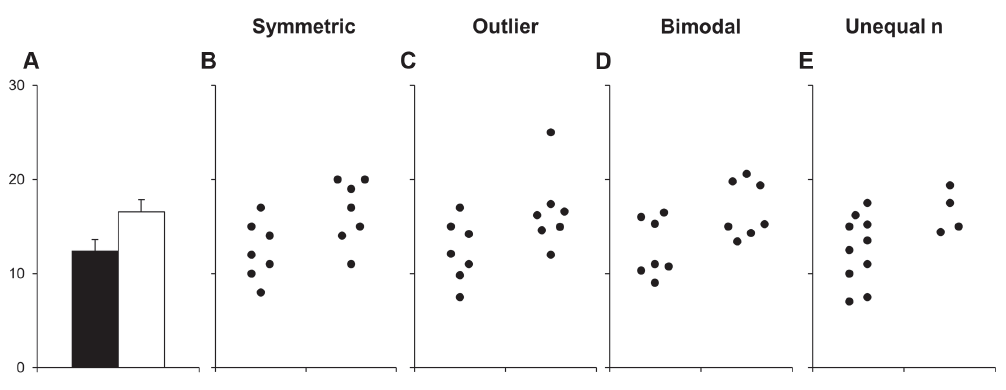
\includegraphics[width=1\textwidth]{images/weissgerber2}  
\end{frame}

% BARS MAY NOT GIVE GOOD STATISTICAL COMPARISONS
\begin{frame}
  \frametitle{Bars may mislead on statistics
  \footnote{\tiny{\href{http://dx.doi.org/10.1371/journal.pbio.1002128}{Weissgerber \textit{et al.} (2015) \textit{PLoS Biol.} doi:10.1371/journal.pbio.1002128}}}
  }
    \begin{alertblock}{Bars may imply incorrect test statistics:}
      Overlaps, outliers, covariates, sample sizes masked
    \end{alertblock}
    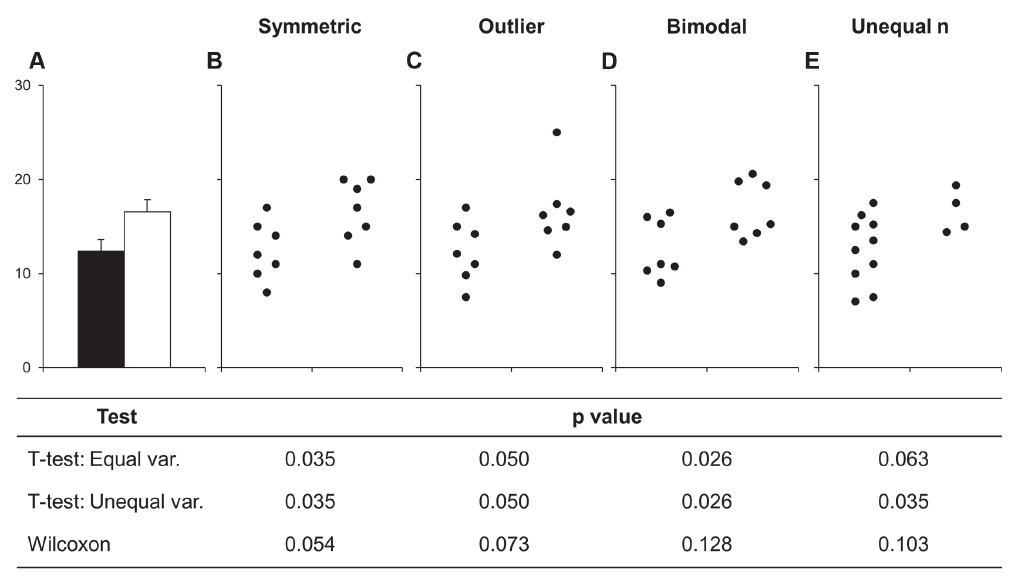
\includegraphics[width=1\textwidth]{images/weissgerber3}  
\end{frame}

% BARS DO NOT SHOW PAIRED DATA WELL
\begin{frame}
  \frametitle{Bars for paired data
  \footnote{\tiny{\href{http://dx.doi.org/10.1371/journal.pbio.1002128}{Weissgerber \textit{et al.} (2015) \textit{PLoS Biol.} doi:10.1371/journal.pbio.1002128}}}
  }
    \begin{alertblock}{Bars imply independence of data:}
    \end{alertblock}
    \begin{center}
      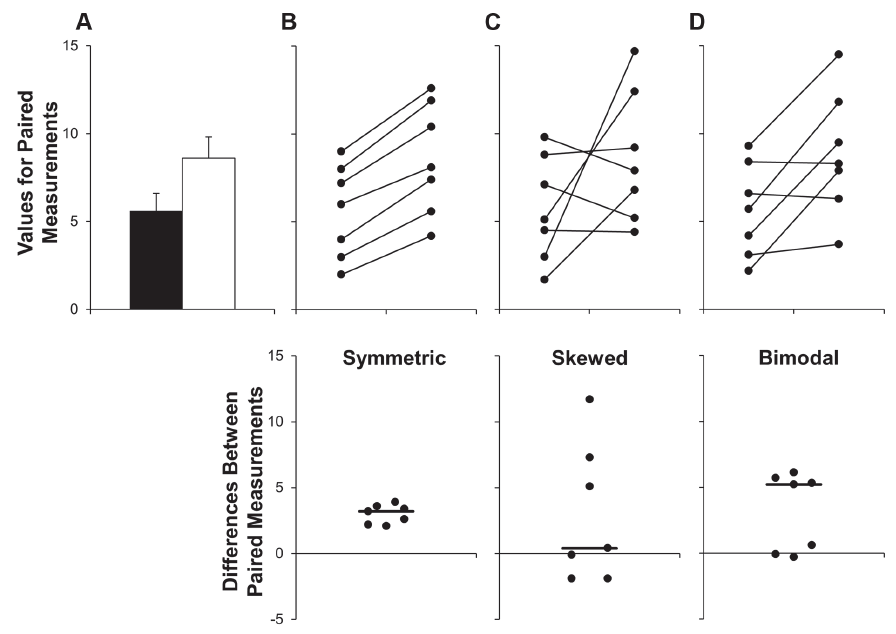
\includegraphics[width=0.8\textwidth]{images/weissgerber4}  
    \end{center}
\end{frame}

% BAR V SCATTER 1
\begin{frame}
  \frametitle{Better than bar charts?}
  \textcolor{hutton_green}{Bar chart with SE bars suggests group 2 is highest}
    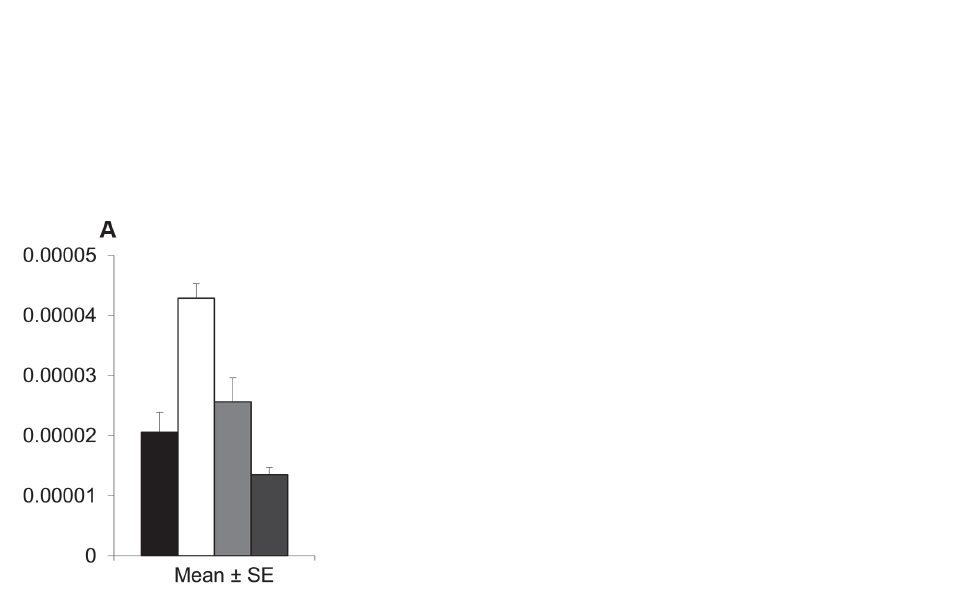
\includegraphics[width=1\textwidth]{images/weissgerber_bar_scatter1}    
\end{frame}

% BAR V SCATTER 2
\begin{frame}
  \frametitle{Better than bar charts?}
  \textcolor{hutton_blue}{Bar chart with SD bars suggests there is overlap}
    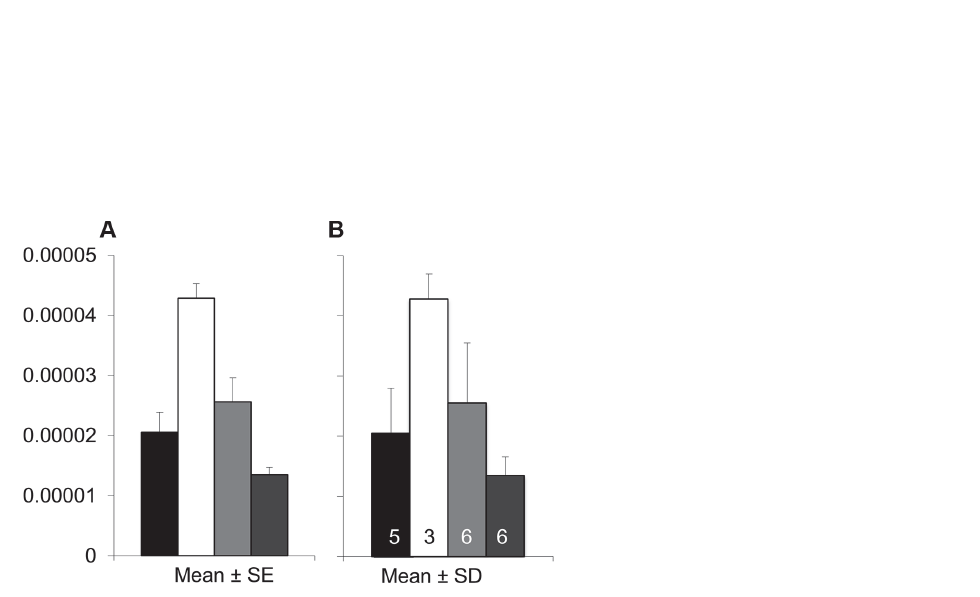
\includegraphics[width=1\textwidth]{images/weissgerber_bar_scatter2}    
\end{frame}

% BAR V SCATTER 3
\begin{frame}
  \frametitle{Better than bar charts?}
  \textcolor{hutton_purple}{Univariate scatterplots show sample sizes, outliers, variance}
    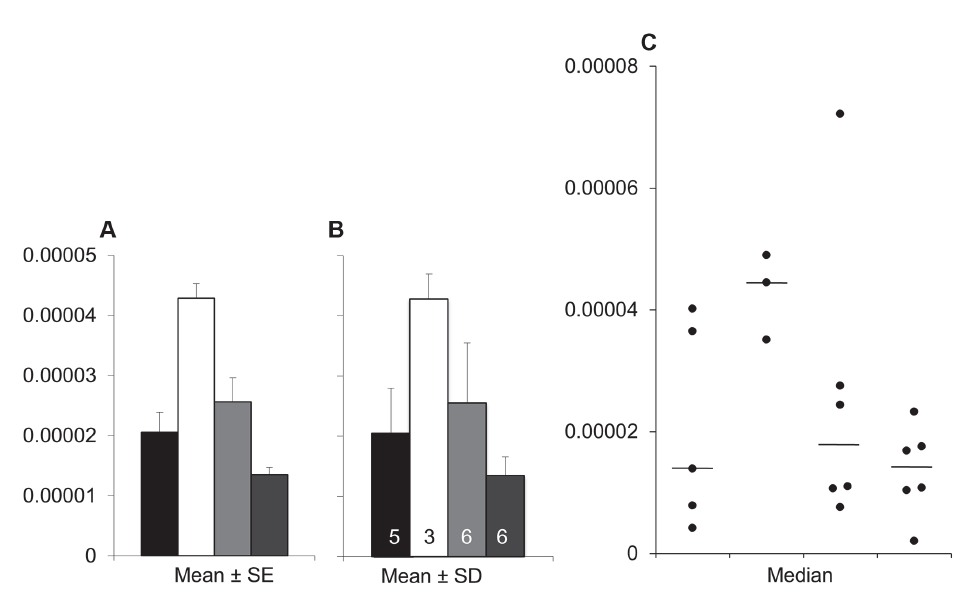
\includegraphics[width=1\textwidth]{images/weissgerber_bar_scatter3}    
\end{frame}